\documentclass[12pt, a4paper]{article} 
 
\usepackage[utf8]{inputenc}
 

\usepackage[bottom = 8em]{geometry} % to change the page dimensions
\geometry{a4paper} % or letterpaper (US) or a5paper or....
 
\usepackage{graphicx} % support the \includegraphics command and options
\usepackage{grffile}
 
\usepackage{booktabs} % for much better looking tables
\usepackage{array} % for better arrays (eg matrices) in maths
\usepackage{float}
\usepackage{paralist} % very flexible & customisable lists (eg. enumerate/itemize, etc.)
\usepackage{verbatim} % adds environment for commenting out blocks of text & for better verbatim
\usepackage{subfig} % make it possible to include more than one captioned figure/table in a single float
% These packages are all incorporated in the memoir class to one degree or another...
 
 
 
\usepackage{amsmath, amssymb}% for mathematical symbols
\usepackage[colorlinks=true,linkcolor=black]{hyperref} % for hyperreferences with black color
%\usepackage[T1]{fontenc} % Uncomment for norwegian document
%\usepackage[norsk]{babel} %
 
%%% HEADERS & FOOTERS
\usepackage{fancyhdr} % This should be set AFTER setting up the page geometry
\pagestyle{fancy} % options: empty , plain , fancy
\renewcommand{\headrulewidth}{0pt} % customise the layout...
\lhead{}\chead{}\rhead{}
\lfoot{}\cfoot{\thepage}\rfoot{}

 
%%% SECTION TITLE APPEARANCE
\usepackage{sectsty}
\allsectionsfont{\sffamily\mdseries\upshape} % (See the fntguide.pdf for font help)
% (This matches ConTeXt defaults)
 
%%% ToC (table of contents) APPEARANCE
\usepackage[nottoc,notlof,notlot]{tocbibind} % Put the bibliography in the ToC
\usepackage[titles,subfigure]{tocloft} % Alter the style of the Table of Contents
\renewcommand{\cftsecfont}{\rmfamily\mdseries\upshape}
\renewcommand{\cftsecpagefont}{\rmfamily\mdseries\upshape} % No bold!
 
 
%%% END Article customizations
 
%%% The "real" document content comes below...
 
\title{Subsymbolic AI assignment 1}
\author{Eivind Hærum \& \ Hong-Dang Lam}
\date{\today} % Activate to display a given date or no date (if empty),
         % otherwise the current date is printed 
 
\begin{document}
\maketitle
%\begin{abstract}
% 
%Abstract
% 
%\end{abstract}
 
\newpage
\tableofcontents
\newpage

\section{Implementation of the proposed system}
Modifications and translation of the provided code etc.

\subsection{System}
The system consist of a webots simulation which uses a world file provided by the course stab. The world file consists of a food-box inside a closed square arena (4 walls) with 7 e-pucks. The box is emitting light along with another global directional light.

The changes we made to the world file was dimming the directional light a bit so the e-puck bots would be more sensitive to the light emitter from the food source, and we changed the attenuation of the box. The attenuation of a point light is calculated as such: $ att = \frac{1}{x+y*r+z*r^2} $ where $r$ is the distance to the emitter. We changed the value of $x$ to 0 and $z$ to 6 - this is because according to the documentation it is recommended to change default attenuation to $[0,0,4\pi]$ which is more realistic, but $4\pi$ is too high for the bots to efficiently find the light source. 
\subsection{Box pushing}
%Implement control system for the box pushing task as provided in the assignment text and
%describe the expected and unexpected behaviours observed during simulation.
The bots uses the distance sensor in the search behavior where they walk aimlessly around searching for the food source. Whenever they see the box/food in front of them they will start the retrieval behavior which uses the light sensors to locate the box (this is possible because it is emitting light). The light sensors gives lower value if it detects stronger lights, and higher valuer otherwise.
The e-pucks only uses the light sensor [0,1,6,7] which are the four sensors in front of it. We are using the different behaviours for this assignment, search, retrieval and stagnation as provided in the .c files.
The search behaviour makes the bots search aimlessly around without colliding into each other while the retrieval will make the bots converge to the box if it can find a light source. After the converging is done the retrieval behaviour intiates a push box behaviour. If the bots are stuck pushing the box for a while without any results it'll try to realign itself so the pushing becomes more effective. If it have tried to realign two times a "find new spot" command is issued. This makes the bot drive in a sequence of move to let it find the left or the right side of the box.
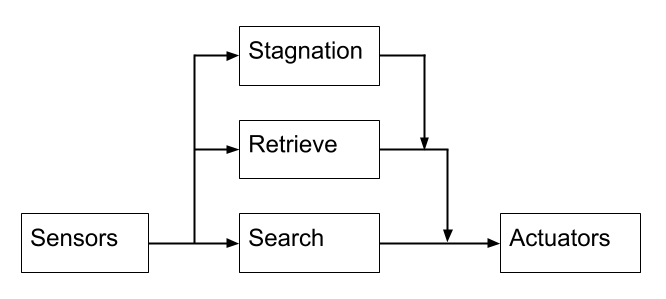
\includegraphics[width=15cm]{Brooks-lite.png}


\section{Discovered weaknesses}
 %Identify areas of the system that may be improved in the single box scenario. These areas may be in overall architecture of controller or at the individual sub-behaviour task. Provide suggestions (one or more) to address these improvements

The stagnation file provided doesn't differentiate between whether the bot is close to the box or not - this led to the bots trying to find new spot before it even tried to push the box. We had to check this ourselves by using the distance sensors in the front. 
The bots doesn't always accomplish the mission either, they tend to get stuck now and then. This usually happens when there's two or three bots on both opposite side of the box. Both "team" think they are pushing the box, and they trust their neighbour. 
\subsection{Possible improvements}

\subsection{Results from the changes made based upon our improvements}
When we implemented the distance checking before changing to stagnation behavior it was able to push the box into the wall.

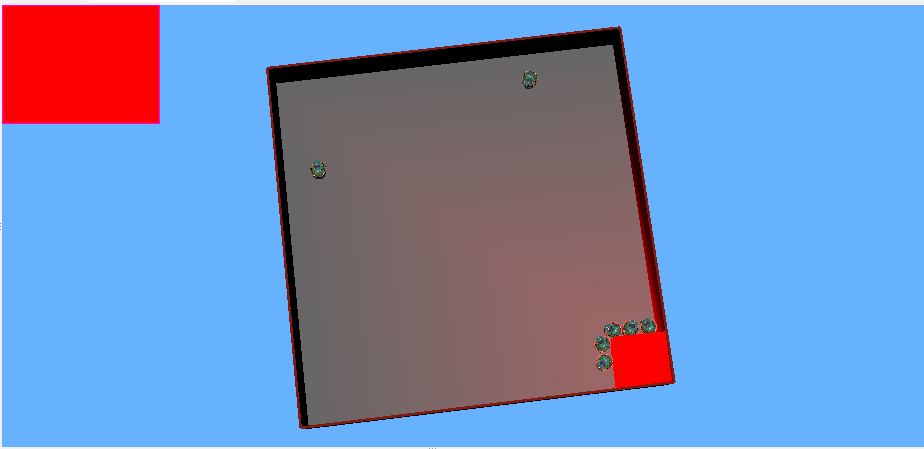
\includegraphics[width=15cm]{1.finalState}


\section{Advanced features}
%TODO

\subsection{New architecture}
\subsection{Modifications}


\end{document}
